\documentclass[11pt]{article}

\usepackage[T1]{fontenc}
\usepackage[utf8]{inputenc}
\usepackage[a4paper,margin=1in]{geometry}
\usepackage{amsmath,amssymb}
\usepackage{graphicx}
\usepackage{booktabs}
\usepackage{xcolor}
\usepackage{caption}
\usepackage{listings}
\usepackage{mdframed}
\usepackage[authoryear,round]{natbib}
\usepackage[colorlinks=true,linkcolor=blue!50!black,citecolor=blue!50!black,urlcolor=blue!50!black]{hyperref}

\definecolor{codebg}{gray}{0.96}
\definecolor{codekw}{rgb}{0.0,0.3,0.6}
\definecolor{codecm}{rgb}{0.3,0.5,0.3}
\lstset{
  basicstyle=\ttfamily\small,
  backgroundcolor=\color{codebg},
  keywordstyle=\color{codekw}\bfseries,
  commentstyle=\color{codecm}\itshape,
  breaklines=true,
  showstringspaces=false,
  frame=single,
  framesep=4pt,
  language=Python,
  columns=fullflexible,
}

\newmdenv[linecolor=blue!40!black,linewidth=0.8pt,backgroundcolor=blue!3,
          skipabove=8pt,skipbelow=8pt,innertopmargin=6pt,innerbottommargin=6pt]{keybox}
\newmdenv[linecolor=orange!60!black,linewidth=0.8pt,backgroundcolor=orange!5,
          skipabove=8pt,skipbelow=8pt,innertopmargin=6pt,innerbottommargin=6pt]{qbox}

\newcommand{\R}{\mathbb{R}}
\newcommand{\E}{\mathbb{E}}
\newcommand{\Var}{\operatorname{Var}}
\newcommand{\rlm}{r_{\ell m}}
\newcommand{\code}[1]{\texttt{#1}}

\title{\textbf{Trainable, Differentiable SPPT}\\[4pt]
\large A student's guide to learning the parameters of a stochastic weather model
by gradient descent}
\author{Stochastic parametrization tutorial \\ \code{examples/stochastic\_sppt/}}
\date{\today}

\begin{document}
\maketitle

\begin{abstract}
\noindent
This document is a self-contained tutorial for a reader who has taken a first
course in atmospheric dynamics and knows some Python, but who has \emph{not}
necessarily seen ensemble forecasting, proper scoring rules, or stochastic
gradient estimation. We build a stochastic version of an idealised
(Held--Suarez) atmospheric model using \textbf{SPPT} --- Stochastically
Perturbed Parametrization Tendencies --- and then \emph{learn} the three
parameters that control the stochasticity by \textbf{gradient descent through the
model}. Because the entire model is written as a differentiable \code{JAX}
program, we can compute the derivative of an ensemble forecast score with respect
to the noise parameters and optimise them. We explain every ingredient from
first principles: the perturbation scheme, the spectral pattern generator, how
``truth'' data is generated and stored, the scoring rule (CRPS and its
finite-ensemble corrections), the calibration diagnostics (spread--error ratio,
rank histogram), and --- in detail --- \emph{how one differentiates through
randomness and what the gradient is taken with respect to}. We show the results
of the first milestone (parameter recovery), discuss honestly where and why the
recovered value departs from the truth, and give exercises and further reading.
\end{abstract}

\tableofcontents

%==============================================================================
\section{Why a weather model needs randomness}
%==============================================================================

A weather or climate model integrates the equations of motion on a grid. Motions
smaller than the grid box --- convection, turbulence, cloud microphysics, gravity
waves --- cannot be resolved, so their \emph{average} effect on the resolved flow
is supplied by \emph{parametrizations}: deterministic formulas that return a
tendency (a rate of change $\partial X/\partial t$) for each prognostic variable
$X$. These formulas are approximations with real, structural uncertainty: two
defensible convection schemes disagree, and neither is ``correct''.

A single deterministic forecast hides this uncertainty. An \textbf{ensemble
forecast} exposes it: run the model many times with slightly different
initial conditions and/or slightly perturbed physics, and the \emph{spread} of the
resulting forecasts is an estimate of the forecast uncertainty. For the ensemble
to be trustworthy it must be \textbf{reliable} (also called
\emph{calibrated}): on the occasions when the ensemble is confident (small
spread) it should usually be right, and when it is uncertain (large spread) the
truth should more often be far from the mean. Quantifying and achieving
reliability is the technical heart of this tutorial.

\textbf{SPPT} \citep{palmer2009} represents model uncertainty by multiplying the
\emph{total parametrized physics tendency} by a smoothly varying random field.
If the deterministic physics returns a tendency $P_X$ for variable $X$, SPPT
replaces it with
\begin{equation}
  \tilde P_X(\mathbf{x},z,t) \;=\; \bigl(1 + \mu(z)\, r(\mathbf{x},t)\bigr)\, P_X(\mathbf{x},z,t),
  \label{eq:sppt}
\end{equation}
where $r(\mathbf{x},t)$ is a random pattern that is smooth in space and
correlated in time, $\mu(z)\in[0,1]$ is a vertical taper (SPPT is switched off
near the surface and in the stratosphere, where the multiplicative assumption is
poor), and the same $r$ multiplies the wind and temperature tendencies at a given
column so that the perturbation is physically consistent. Different draws of $r$
give different ensemble members.

\begin{keybox}
\textbf{The idea of this project.} The pattern $r$ is controlled by three numbers:
its amplitude $\sigma$, its temporal decorrelation time $\tau$, and its spatial
correlation length $\ell$. Normally these are hand-tuned. Here the model is
\emph{differentiable}, so we instead \textbf{learn} $(\sigma,\tau,\ell)$ by
minimising an ensemble forecast score with gradient descent. Reproducing SPPT
and the score faithfully is standard; the \emph{trainable / differentiable}
framing is the contribution.
\end{keybox}

%==============================================================================
\section{The deterministic core}
%==============================================================================

The host model is a dry primitive-equation spectral dynamical core forced by the
\citet{heldsuarez1994} benchmark: Newtonian relaxation of temperature towards a
prescribed radiative-equilibrium profile and Rayleigh damping of low-level winds.
Held--Suarez is a standard idealisation --- it produces a realistic midlatitude
jet and baroclinic eddies without any moisture or radiation code --- so it is the
perfect laboratory for a methods paper: cheap, reproducible, and free of
confounding physics. In the code the Held--Suarez forcing plays the role of ``the
parametrized physics'' $P_X$ that SPPT perturbs (\code{held\_suarez.py}).

The dynamics are \emph{spectral}: the prognostic fields are represented by their
spherical-harmonic coefficients and truncated triangularly at total wavenumber
$T$ (``T21'' means $T=21$). We run at several resolutions
(Table~\ref{tab:res}); the differentiable training in this tutorial is done at
\textbf{T21} for reasons explained in \S\ref{sec:hardware}.

\begin{table}[h]
\centering
\caption{Resolutions (\code{config.py}). $L$ is the spherical-harmonic bandlimit
($n_{\text{lat}}=L$, $n_{\text{lon}}=2L-1$); $T$ is the triangular truncation;
$\Delta t$ is the time step (chosen for numerical stability).}
\label{tab:res}
\begin{tabular}{lccc}
\toprule
name & $L$ & $T$ & $\Delta t$ (s) \\
\midrule
T21  & 32  & 21  & 1800 \\
T42  & 64  & 42  & 1200 \\
T85  & 128 & 85  & 600  \\
T127 & 192 & 127 & 450  \\
\bottomrule
\end{tabular}
\end{table}

Everything --- dynamics, physics, SPPT, and the score --- is a pure \code{JAX}
function, so it can be composed with \code{jax.jit} (compile), \code{jax.vmap}
(vectorise over ensemble members), and, crucially, \code{jax.grad} (automatic
differentiation). That last property is what makes training possible.

\begin{keybox}
\textbf{Float64 is mandatory.} Spectral dynamics are numerically stiff; single
precision silently corrupts them. Every entry point forces
\code{JAX\_ENABLE\_X64=True}. On Apple Silicon, \code{JAX} defaults to a Metal
backend that \emph{cannot} do float64, so we also pin \code{JAX\_PLATFORMS=cpu}
(a cluster's CUDA setting still wins). If you forget this, you will get either a
crash or, worse, quietly wrong numbers.
\end{keybox}

%==============================================================================
\section{The stochastic pattern generator}\label{sec:pattern}
%==============================================================================

The pattern $r$ is built in \emph{spectral} space, because there its statistics
(variance and correlation length) are set analytically. This follows Appendix~8.1
of \citet{palmer2009}.

\subsection{A first-order autoregressive process, one coefficient at a time}

Each spherical-harmonic coefficient $\rlm$ (degree $\ell$, order $m$) evolves as
an independent complex \textbf{AR(1)} (first-order autoregressive) process:
\begin{equation}
  \rlm^{(t+\Delta t)} \;=\; \phi\, \rlm^{(t)} \;+\; \sigma_\ell\, \eta_{\ell m}^{(t)},
  \qquad
  \phi = e^{-\Delta t/\tau},
  \label{eq:ar1}
\end{equation}
where $\eta_{\ell m}^{(t)}$ are i.i.d.\ complex standard Gaussians (real and
imaginary parts $\sim\mathcal N(0,1)$), and $\sigma_\ell$ is a forcing amplitude
that depends only on the total wavenumber $\ell$. Equation~\eqref{eq:ar1} is the
discrete analogue of an Ornstein--Uhlenbeck process: $\phi$ close to $1$ (large
$\tau$) means the pattern changes slowly; $\phi$ close to $0$ (small $\tau$) means
it is refreshed every step.

\paragraph{Stationary variance.} Taking the variance of \eqref{eq:ar1} in the
stationary state ($\Var[\rlm^{(t+\Delta t)}]=\Var[\rlm^{(t)}]=:v_\ell$) and using
independence of $\eta$ from $r$,
\begin{equation}
  v_\ell = \phi^2 v_\ell + \sigma_\ell^2\,\underbrace{\Var[\eta]}_{=1}
  \quad\Longrightarrow\quad
  v_\ell = \frac{\sigma_\ell^2}{1-\phi^2}.
  \label{eq:statvar}
\end{equation}
This is why the code \emph{initialises} the coefficients from
$\rlm^{(0)} = (1-\phi^2)^{-1/2}\,\sigma_\ell\,\eta_{\ell m}$: it starts the process
already in its stationary distribution, so there is no spin-up transient.

\subsection{Setting the amplitude and the length scale}

The forcing amplitude has a shape in wavenumber and an overall scale:
\begin{equation}
  \sigma_\ell = F_0\, \exp\!\Bigl(-\tfrac{1}{2}\,\kappa_T\,\ell(\ell+1)\Bigr),
  \qquad
  \kappa_T = \frac{1}{2}\left(\frac{\ell_{\text{corr}}}{a}\right)^{2},
  \label{eq:sigmaell}
\end{equation}
where $a$ is the planetary radius and $\ell_{\text{corr}}$ is the physical
correlation length. Because $\ell(\ell+1)$ is the eigenvalue of the Laplacian on
the sphere for degree $\ell$, the factor $\exp(-\tfrac12\kappa_T\,\ell(\ell+1))$
is a Gaussian low-pass filter: large $\ell_{\text{corr}}$ (large $\kappa_T$)
suppresses high wavenumbers and yields a spatially \emph{smooth} pattern with big
features; small $\ell_{\text{corr}}$ lets small scales through.

The overall scale $F_0$ is fixed by demanding that the \emph{grid-point} variance
of $r$ equals the target $\sigma^2$. Summing the stationary variance
\eqref{eq:statvar} over all coefficients (with the $2\ell+1$ multiplicity of
order $m$) and matching gives, up to the transform's normalisation convention,
\begin{equation}
  F_0 = \sqrt{\frac{\;C\,\sigma^2\,(1-\phi^2)\;}
                   {\;2\sum_{\ell\ge 1}(2\ell+1)\,e^{-\kappa_T\,\ell(\ell+1)}\;}},
  \label{eq:F0}
\end{equation}
where $C$ is a single scalar (\code{\_VAR\_NORM}) reconciling the analytic
formula with the particular inverse-transform convention of the spherical-harmonic
library. In code (\code{sppt.py}):

\begin{lstlisting}
def sigma_n(params, trans_config, dt):
    L, radius = trans_config.L, trans_config.radius
    n = jnp.arange(L)                                   # total wavenumber l
    kappa_t = (jnp.exp(params.log_len) / radius) ** 2 / 2.0
    shape = jnp.exp(-kappa_t * n * (n + 1) / 2.0)       # eq. (3): the l-shape
    var_r = jnp.exp(2.0 * params.log_sigma)             # sigma^2
    phi   = jnp.exp(-dt / jnp.exp(params.log_tau))
    denom = 2.0 * jnp.sum((2*n[1:]+1) * jnp.exp(-kappa_t * n[1:]*(n[1:]+1)))
    F0 = jnp.sqrt(_VAR_NORM * var_r * (1.0 - phi**2) / denom)
    return F0 * shape                                   # sigma_l, shape (L,)
\end{lstlisting}

Finally an inverse spherical-harmonic transform turns the coefficients $\rlm$
into a real field $r(\mathbf x)$ on the grid, which enters \eqref{eq:sppt}. The
pattern is clipped at $\pm 3\sigma$ and the multiplicative factor
$1+\mu r$ is clipped to $[0.1,1.9]$, both standard safeguards from
\citet{palmer2009} that keep a rare large draw from flipping the sign of a
tendency.

\begin{keybox}
\textbf{An honest caveat about $\sigma$ (\code{sppt.py}).} The normalisation
constant $C$ is calibrated \emph{once}, at T21. The transform convention is not
exactly resolution-independent, so at T42 and finer the true grid-point standard
deviation is about $1.12\times\sigma$. This does \emph{not} affect anything in
this tutorial: parameter recovery is done entirely at T21, and even at other
resolutions the constant cancels between the ``truth'' model and the forecast
model (they share the code). Only the \emph{physical interpretation} of a learned
$\sigma$ carries the offset. We leave it constant deliberately, to watch how the
optimiser tunes the \emph{effective} $\sigma$.
\end{keybox}

The three parameters are stored in \textbf{log space}, so that gradient steps can
never make them non-physical (negative), and so that a multiplicative change is a
fixed additive step regardless of scale:
\begin{lstlisting}
class SPPTParams:
    log_sigma   # sigma = exp(log_sigma), grid-point std of r     (default 0.5)
    log_tau     # tau   = exp(log_tau),   decorrelation time (s)  (default 6 h)
    log_len     # ell   = exp(log_len),   correlation length (m)  (default 500 km)
\end{lstlisting}

%==============================================================================
\section{Generating and storing the ``truth''}\label{sec:data}
%==============================================================================

To \emph{learn} the parameters we need something to score the forecast against.
This tutorial uses the cleanest possible setup, an \textbf{identical-twin}
experiment (Mode~A, milestone~M1):

\begin{enumerate}
\item Pick a set of initial conditions (``cases''). We spin the deterministic
  model up for 120--200 days to reach a statistically steady midlatitude flow,
  then sample $N_c$ atmospheric states a few days apart. Each sampled state is
  one case's initial condition.
\item For each case, run the \emph{stochastic} model forward with a \emph{known}
  set of parameters $\theta^\star=(\sigma=0.5,\ \tau=6\,\text{h},\
  \ell=500\,\text{km})$ and save the state at each lead time. That saved
  trajectory is the ``truth'' $y$ for that case.
\item Start the optimiser from a deliberately \emph{wrong} guess and check that it
  recovers $\theta^\star$.
\end{enumerate}

Because the ``truth'' is generated by the \emph{same model} we will forecast with,
there is \emph{no model error} --- only the parameters differ. This isolates the
learning machinery. (Mode~B, where the truth is a higher-resolution run and SPPT
must compensate genuine model error, is the harder, later milestone.)

\paragraph{What is stored, and in what shape.} A dataset
(\code{generate\_data.py}) is a dictionary saved with \code{pickle}:
\begin{lstlisting}
{
  "ic_specs": SpectralState,          # the N_c initial conditions (spectral)
  "truth":   {field: array[N_c, n_lead, lat, lon]},  # 5 verification fields
  "lead_steps": (steps_per_lead, ...),
  "forecast_resolution": "T21", "n_lev": 20,
}
\end{lstlisting}
The five verification fields are \code{u850}, \code{v850} (winds at 850\,hPa),
\code{t500} (temperature at 500\,hPa), \code{vort500} (relative vorticity at
500\,hPa) and \code{ps} (surface pressure) --- a small, standard set spanning the
mass and wind fields at low and mid levels. Each is diagnosed from the spectral
state by transforming to the grid and interpolating in log-pressure
(\code{diagnostics.py}). The initial conditions are stored in spectral space
(they are the exact model state); the truth is stored as grid-space verification
fields (that is what we score).

\begin{qbox}
\textbf{Design question (raised by a careful reader): why only \emph{one}
stochastic run per initial condition? If I ran the model several times from the
same IC and stored each as a separate target, would training improve --- and at
what cost?}

\smallskip\noindent
\emph{Short answer: yes, it would reduce the small bias discussed in
\S\ref{sec:whybias}, it is cheap at training time, and it costs storage and
truth-generation time linear in the number of draws. Here is why.}

\smallskip\noindent
For a fixed initial condition the ``truth'' is itself a \emph{random} draw
$y\sim F^\star$ from the true forecast distribution (the stochastic model with
$\theta^\star$). The quantity we would \emph{like} to minimise is the expected
score $\E_{y\sim F^\star}[\,\mathrm{CRPS}(F_\theta, y)\,]$. With a single stored
truth draw we replace that expectation by a one-sample estimate
$\mathrm{CRPS}(F_\theta, y_1)$, which is noisy and slightly biased. If instead we
store $K$ independent truth draws $y_1,\dots,y_K$ from the same IC and average,
\begin{equation}
  \frac{1}{K}\sum_{k=1}^{K}\mathrm{CRPS}(F_\theta, y_k)
  \;\xrightarrow[K\to\infty]{}\;
  \E_{y\sim F^\star}[\mathrm{CRPS}(F_\theta, y)],
\end{equation}
the estimate's variance falls like $1/K$ and its minimiser moves towards
$\theta^\star$.

\smallskip\noindent
\textbf{Cost.} The \emph{expensive} object in a training step is the forecast
ensemble rollout $F_\theta$ (a reverse-mode-differentiated integration; see
\S\ref{sec:memory}). That rollout is computed \emph{once per case} and can be
scored against all $K$ truth draws --- the extra $K-1$ comparisons are just
cheap CRPS evaluations ($O(M^2)$ arithmetic on already-computed fields), \emph{no
extra model integrations}. So more truth draws barely change the per-step
training time. What they \emph{do} cost is (i) truth-generation time, which is $K$
forward integrations per case, and (ii) storage, $K\times$ the dataset size.
Contrast this with adding more \emph{cases} (distinct ICs), which samples
different weather regimes and reduces a different component of the variance, or
adding more \emph{ensemble members} $M$, which is expensive because it multiplies
the reverse-mode rollout cost. \textbf{Exercise~\ref{ex:multidraw}} asks you to
implement multi-draw truth and measure the effect.
\end{qbox}

\begin{keybox}
\textbf{A known imperfection in Mode~A truth.} The truth generator re-initialises
the SPPT pattern at each lead boundary rather than carrying it continuously. At
$\tau=6$\,h with multi-day leads this is numerically inert ($\phi^{n}\!\sim\!10^{-4}$
between leads --- the pattern has fully decorrelated, so a fresh stationary draw
is statistically identical to a carried one). It would matter for long $\tau$ or
sub-daily leads, and is flagged in the log as a follow-up.
\end{keybox}

%==============================================================================
\section{Scoring an ensemble: the CRPS}\label{sec:crps}
%==============================================================================

We need a single number measuring how well an ensemble forecast matches a scalar
truth $y$, such that the number is minimised (in expectation) exactly when the
forecast distribution equals the true one. Such a \textbf{proper scoring rule} is
the \emph{Continuous Ranked Probability Score} \citep{gneiting2007}. For a
predictive distribution with CDF $F$ and an observation $y$,
\begin{equation}
  \mathrm{CRPS}(F,y) = \int_{-\infty}^{\infty}\!\bigl(F(x) - \mathbf 1\{x\ge y\}\bigr)^2\,dx
  \;=\;
  \E_F|X-y| - \tfrac12\,\E_F|X-X'|,
  \label{eq:crps}
\end{equation}
where $X,X'$ are independent draws from $F$. The second form is the useful one for
ensembles: the first term rewards putting mass near $y$; the second term
($-\tfrac12$ mean pairwise distance) rewards \emph{sharpness} but penalises
overconfidence, and it is what makes CRPS proper --- it is minimised when $F=F^\star$.

\paragraph{The finite-ensemble bias, and the ``fair'' fix.} With only $M$ members
$x_1,\dots,x_M$ the natural plug-in estimator uses
$\tfrac{1}{M^2}\sum_{i,j}|x_i-x_j|$ for the second term. This
\emph{under}-estimates the pairwise spread of the underlying distribution (it
includes the $M$ zero terms $|x_i-x_i|$ and uses the biased $1/M^2$ normaliser),
so it \emph{rewards} an ensemble that is too narrow: a small ensemble looks
artificially good. The \textbf{fair CRPS} \citep{leutbecher2018,lang2024} removes
this by using the unbiased pairwise estimator $\tfrac{1}{M(M-1)}\sum_{i\ne j}$:
\begin{equation}
  \mathrm{fCRPS} = \frac{1}{M}\sum_{i=1}^{M}|x_i-y|
    \;-\; \frac{1}{2M(M-1)}\sum_{i=1}^{M}\sum_{j=1}^{M}|x_i-x_j|.
  \label{eq:faircrps}
\end{equation}
Fair CRPS estimates the score the \emph{infinite} ensemble would get, so it does
not reward under-dispersion; it is the correct target when training an ensemble
system to be reliable. The \textbf{almost-fair} variant \citep{lang2024}
interpolates with a parameter $\alpha\in[0,1]$,
\begin{equation}
  \mathrm{afCRPS} = \frac{1}{M}\sum_i |x_i-y|
    \;-\; \frac{1-\epsilon}{2M(M-1)}\sum_{i,j}|x_i-x_j|,
  \qquad \epsilon=\frac{1-\alpha}{M},
  \label{eq:afcrps}
\end{equation}
with $\alpha=1$ giving fair CRPS. The small $\epsilon$ avoids a degeneracy Lang
et al.\ identified when training (it keeps a slight preference for finite spread,
which stabilises early optimisation). We use $\alpha=0.95$. In code
(\code{metrics.py}), vectorised over grid points:
\begin{lstlisting}
def afcrps(ensemble, truth, alpha=0.95):        # ensemble: (M, ...), truth: (...)
    M = ensemble.shape[0]
    eps = (1.0 - alpha) / M
    e1 = jnp.mean(jnp.abs(ensemble - truth[None]), axis=0)       # skill term
    diff = jnp.abs(ensemble[:, None] - ensemble[None, :])        # (M, M, ...)
    e2 = jnp.sum(diff, axis=(0, 1)) / (2.0 * M * (M - 1))        # fair spread term
    return jnp.mean(e1 - (1.0 - eps) * e2)
\end{lstlisting}
The training loss aggregates afCRPS over cases, lead times, and the five fields,
each field normalised by its truth standard deviation so that surface pressure
(in Pa, $O(10^3)$) does not dominate temperature (in K, $O(10)$):
\begin{equation}
  J(\theta) = \frac{1}{5}\sum_{f\in\text{fields}}
    \frac{1}{s_f}\;
    \frac{1}{N_c N_\ell}\sum_{c,\lambda}
    \mathrm{afCRPS}\!\bigl(F_\theta^{c,\lambda,f},\, y^{c,\lambda,f}\bigr),
  \qquad s_f=\operatorname{std}(y^f).
  \label{eq:loss}
\end{equation}

%==============================================================================
\section{Is the ensemble calibrated? Two diagnostics}\label{sec:diag}
%==============================================================================

A low score is necessary but not transparent. Two classical diagnostics
\emph{visualise} reliability directly.

\subsection{Spread--error ratio}\label{sec:spreaderror}

Intuitively, a reliable ensemble's spread should match the error of its mean: if
the members scatter with standard deviation $s$, the truth should typically sit
about $s$ away from the ensemble mean. The precise statement carries a
finite-ensemble correction that is easy to derive.

Suppose the ensemble is \emph{reliable} in the strong sense that the truth $y$ and
the $M$ members $x_1,\dots,x_M$ are \textbf{exchangeable} --- all $M{+}1$ are
i.i.d.\ draws from a common distribution with variance $\sigma_c^2$ about a common
mean. Write $\bar x=\tfrac1M\sum_i x_i$ and the sample variance
$s^2=\tfrac{1}{M-1}\sum_i (x_i-\bar x)^2$. Then
\begin{align}
  \E[s^2] &= \sigma_c^2, \label{eq:Es2}\\
  \E\bigl[(y-\bar x)^2\bigr] &= \Var(y) + \Var(\bar x)
     = \sigma_c^2 + \frac{\sigma_c^2}{M} = \frac{M+1}{M}\,\sigma_c^2,
     \label{eq:Eerr}
\end{align}
using independence of $y$ from the members and $\Var(\bar x)=\sigma_c^2/M$.
Dividing \eqref{eq:Eerr} by \eqref{eq:Es2},
\begin{equation}
  \E\bigl[(y-\bar x)^2\bigr] = \frac{M+1}{M}\,\E[s^2]
  \quad\Longrightarrow\quad
  \boxed{\ \text{ratio} \;=\; \sqrt{\tfrac{M+1}{M}}\;\frac{\text{spread}}{\text{rmse}} \;=\; 1\ }
  \label{eq:sprerr}
\end{equation}
for a reliable ensemble \citep{fortin2014,leutbecher2018}, where
$\text{spread}=\sqrt{\E[s^2]}$ (root-mean ensemble variance) and
$\text{rmse}=\sqrt{\E[(y-\bar x)^2]}$ (root-mean-square error of the mean). The
$\sqrt{(M{+}1)/M}$ factor is the correction for the fact that a finite ensemble
mean is itself uncertain; forgetting it makes every finite ensemble look slightly
under-dispersed. A ratio \emph{below} 1 means the ensemble is
\textbf{under}-dispersed (overconfident: errors exceed the spread); \emph{above}
1 means \textbf{over}-dispersed. The code (\code{metrics.py}) pools the
expectations over cases and grid points:
\begin{lstlisting}
def spread_error_ratio(ensemble, truth):        # -> 1 for a reliable ensemble
    M = ensemble.shape[0]
    return jnp.sqrt((M + 1.0) / M) * spread(ensemble) / rmse_of_mean(ensemble, truth)
\end{lstlisting}

\begin{keybox}
\textbf{Validate the diagnostic, not just the code.} The first version of this
diagnostic (and its unit test) used a wrong formula that nonetheless
\emph{passed} against a mis-constructed test scenario. The fix was to build a
genuinely exchangeable ensemble in the test (truth and members all i.i.d.\ from
one centre) and confirm the ratio is $\approx 1$ (measured 1.013). Lesson: a test
that passes against the wrong scenario proves nothing --- check that the scenario
itself encodes the property you are testing.
\end{keybox}

\subsection{Rank histogram (Talagrand diagram)}\label{sec:rankhist}

The rank histogram \citep{hamill2001} checks reliability without assuming
Gaussianity. For each verification point, pool the $M$ members and the truth,
sort them, and record the \textbf{rank} of the truth among the members: the number
of members below it, an integer in $\{0,1,\dots,M\}$ ($M{+}1$ possible values).
If the truth is statistically indistinguishable from a member (the ideal), it is
equally likely to fall in any of the $M{+}1$ gaps, so \textbf{the histogram of
ranks over many points is flat}. Departures from flat have textbook shapes:

\begin{table}[h]
\centering
\caption{Reading a rank histogram.}
\label{tab:rank}
\begin{tabular}{ll}
\toprule
shape & interpretation \\
\midrule
flat (uniform)            & calibrated --- truth behaves like a member \\
$\cup$ (U-shaped)         & \textbf{under}-dispersed: truth too often an outlier (rank 0 or $M$) \\
$\cap$ (dome)             & \textbf{over}-dispersed: truth too often central \\
sloped / asymmetric       & \textbf{biased}: forecast systematically off to one side \\
\bottomrule
\end{tabular}
\end{table}

\begin{lstlisting}
def rank_histogram(ensemble, truth):            # length M+1
    rank = jnp.sum(ensemble < truth[None], axis=0).ravel()   # 0..M per point
    return jnp.bincount(rank, length=ensemble.shape[0] + 1)
\end{lstlisting}
A third, informal check --- overlaying the histogram of the members' anomalies (a
member minus the ensemble mean) with the truth's anomaly --- shows directly
whether the truth ``looks like'' a draw from the ensemble.

%==============================================================================
\section{Learning the parameters: differentiating through randomness}
\label{sec:learn}
%==============================================================================

This is the conceptual core. We want $\nabla_\theta J(\theta)$, the gradient of
the ensemble score \eqref{eq:loss} with respect to
$\theta=(\log\sigma,\log\tau,\log\ell)$. But $J$ is defined through a
\emph{random} object --- the ensemble depends on the noise draws. What does it even
mean to differentiate through randomness, and what is the derivative taken with
respect to?

\subsection{The reparameterization (pathwise) gradient}\label{sec:reparam}

Write the noise used by one ensemble member as $\eta$ --- the whole collection of
i.i.d.\ standard Gaussians drawn for the stationary initialisation and every AR(1)
step \eqref{eq:ar1}. The key observation is that in \eqref{eq:ar1} the noise
$\eta$ is drawn from a \textbf{fixed} distribution ($\mathcal N(0,1)$) that
\emph{does not depend on $\theta$}; all the $\theta$-dependence lives in the
\emph{coefficients} $\phi(\theta)$ and $\sigma_\ell(\theta)$. Therefore a member's
entire trajectory --- and hence each of its five verification fields --- is a
\textbf{deterministic, differentiable function} of $\theta$ once $\eta$ is fixed:
\begin{equation}
  x^{(m)}_\theta = G(\theta, \eta^{(m)}),
  \qquad \eta^{(m)}\sim p(\eta)\ \text{independent of }\theta .
\end{equation}
This is the \textbf{reparameterization trick} (also ``pathwise'' gradient)
\citep{kingma2014,mohamed2020}: instead of sampling $x$ from a
$\theta$-dependent distribution (which we could not differentiate directly), we
sample $\theta$-independent noise $\eta$ and pass it through a differentiable map
$G$. The loss becomes an expectation over the \emph{fixed} noise law,
\begin{equation}
  J(\theta) = \E_{\eta^{(1:M)}\sim p}
     \Bigl[\, \mathrm{afCRPS}\bigl(\{G(\theta,\eta^{(m)})\}_{m=1}^M,\; y\bigr)\Bigr],
\end{equation}
and because the distribution we average over no longer depends on $\theta$, the
gradient passes \emph{inside} the expectation:
\begin{equation}
  \nabla_\theta J
   = \E_{\eta^{(1:M)}}\Bigl[\, \nabla_\theta\,
       \mathrm{afCRPS}\bigl(\{G(\theta,\eta^{(m)})\}, y\bigr)\Bigr].
  \label{eq:pathwise}
\end{equation}
We estimate the expectation \eqref{eq:pathwise} by \textbf{Monte Carlo}: draw one
batch of cases and one set of member noises, and evaluate the bracket. That is a
\emph{stochastic gradient} --- an unbiased, noisy estimate of $\nabla_\theta J$ ---
exactly the kind stochastic optimisers are built for.

\begin{keybox}
\textbf{What is the gradient with respect to?} With respect to the three
\emph{log-parameters} $\theta=(\log\sigma,\log\tau,\log\ell)$ --- numbers, not
fields. \textbf{What flows through it?} Reverse-mode automatic differentiation
(\code{jax.grad}) traces the dependence of the score on $\theta$ backwards
through the afCRPS, through every member's multi-day integration (dynamics $+$
SPPT), and into $\phi(\theta)$ and $\sigma_\ell(\theta)$. \textbf{What is held
fixed?} The noise $\eta$ (the $\mathcal N(0,1)$ draws) and the truth $y$: $y$ is
data, so no gradient flows into it. The afCRPS is built from absolute values
$|x-y|$, which are differentiable everywhere except on a measure-zero set, so the
pathwise gradient is well defined almost surely.
\end{keybox}

\subsection{Common random numbers}\label{sec:crn}

The estimator \eqref{eq:pathwise} is unbiased for \emph{any} way of drawing the
$\eta$. But if we re-drew fresh noise every optimiser step, two nearby $\theta$'s
would be scored with different noise, and the difference in their losses would be
dominated by noise rather than by the change in $\theta$ --- a very high-variance
gradient. We therefore use \textbf{common random numbers}: within a single
gradient evaluation the member noises are fixed (derived deterministically from a
per-step key). This is the Monte Carlo analogue of comparing two policies on the
\emph{same} random scenarios, and it dramatically reduces the variance of the
stochastic gradient. It is essential for optimising a stochastic scheme in
practice.

\begin{lstlisting}
def member_keys(base_key, case_idx, n_members):     # deterministic per (case, member)
    return jax.random.split(jax.random.fold_in(base_key, case_idx), n_members)

# one training step (train.py, condensed):
grad_fn = jax.jit(jax.value_and_grad(loss_fn))      # compile once
for step in range(n_steps):
    idx      = choose_a_random_batch_of_cases(step)
    eval_key = fold_in(base_key, 10_000 + step)     # fixed WITHIN this step -> CRN
    loss, grads = grad_fn(params, ic_specs, truth, idx, ..., eval_key, ...)
    updates, opt_state = optax.adam(lr).update(grads, opt_state)
    params = optax.apply_updates(params, updates)   # gradient DESCENT on theta
\end{lstlisting}

\subsection{Reverse mode, checkpointing, and why we train at T21}
\label{sec:memory}\label{sec:hardware}

Reverse-mode autodiff must store intermediate states of the forward integration
to replay them backwards. A single T42 spectral state is $\sim$10\,MB; a 10-day
rollout is $\sim$720 steps, so one differentiated trajectory needs $\sim$7.5\,GB
--- \emph{per member, per case}. Multiplying by an ensemble batch overflows an
18\,GB laptop. Two mitigations are used and one decision is forced:
\begin{itemize}
\item \textbf{Gradient checkpointing} (\code{jax.checkpoint} around the scan body
  in \code{rollout.py}) stores only a subset of states and recomputes the rest
  during the backward pass --- trading compute for memory.
\item \textbf{Vectorising over members with \code{vmap}} and compiling once with
  \code{jax.jit} keeps the step efficient (compile the graph once, then pay only
  arithmetic per step).
\item \textbf{Resolution.} Even so, differentiable training at T42 is infeasible
  on the laptop, so the milestone-M1 sweep is done at \textbf{T21}, where the
  memory is light. Forward-only diagnostics (no gradient, no stored trajectory)
  are cheap at any resolution. Real T42/T127 \emph{training} belongs on a GPU.
\end{itemize}

\begin{keybox}
\textbf{Reproducibility engineering.} On this machine any single process is
killed after $\sim$10 minutes, and the reverse-mode compile of a 5-day-lead graph
alone takes $\sim$8.5 minutes. Two consequences shaped the runnable pipeline:
(i) the recovery sweep uses a \textbf{1-day lead} (48 T21 steps), whose graph
compiles in seconds --- and since $\sigma$-recovery only needs the ensemble spread
to match the identical-twin truth's spread, the short lead is faithful; (ii) the
sweep \textbf{checkpoints every optimiser step to disk} under a wall-clock budget,
so an interrupted run is resumed by simply re-invoking it. Heavy \code{JAX}
compute runs in the foreground; plotting is a separate pure-\code{numpy} step.
\end{keybox}

\subsection{Why $\sigma$ settles slightly \emph{above} 0.5}\label{sec:whybias}

A natural worry: \emph{will $\sigma$ really converge to the true 0.5?} The honest
answer is: to \emph{near} 0.5, settling a couple of percent \emph{above}, and here
is exactly why. Fair CRPS is a \emph{strictly proper} scoring rule, so the
population objective $\E_{y\sim F^\star}[\mathrm{fCRPS}(F_\theta,y)]$ is minimised
at $F_\theta=F^\star$, i.e.\ at $\theta=\theta^\star$ --- \emph{provided} the
forecast family contains the truth (it does, identical twin) and we optimise the
true expectation. We do not optimise the true expectation; we optimise a finite
sample of it \eqref{eq:loss}. Three finite-sample effects act:
\begin{enumerate}
\item \textbf{Finite members $M$}: removed to first order by the fairness
  correction \eqref{eq:faircrps}. This is the one we \emph{do} fix exactly.
\item \textbf{Finite cases $N_c$}: the sample-average objective is a random
  function whose minimiser scatters around $\theta^\star$.
\item \textbf{One truth draw per case}: each case contributes
  $\mathrm{CRPS}(F_\theta, y_c)$ for a \emph{single} random $y_c$. To keep the
  score low on an outlying $y_c$, the optimiser slightly \emph{inflates} the
  spread --- a small \emph{upward} bias in $\sigma$.
\end{enumerate}
Effects 2 and 3 are \emph{sampling} properties, not bugs, and both shrink as
$N_c$ and the number of truth draws grow (\S\ref{sec:data},
Exercise~\ref{ex:multidraw}). In our run $\sigma$ plateaus at $\approx 0.508$ ---
about $2\%$ high --- entirely consistent with this account.

%==============================================================================
\section{Experimental protocol}\label{sec:protocol}
%==============================================================================

\paragraph{Recovery sweep (training).} T21 identical-twin dataset, seed 0, $N_c=12$
cases, truth generated with $\theta^\star=(\sigma{=}0.5,\tau{=}6\text{h},
\ell{=}500\text{km})$, 1-day lead. We recover $\sigma$ alone (freezing $\tau,\ell$
at truth by masking their gradients) --- the single-parameter problem gives the
cleanest, most interpretable convergence story. Optimiser: Adam
\citep{kingma2015adam}, learning rate $0.03$; batch of 3 cases per step,
$M=4$ members; start from a deliberately wrong $\sigma=0.2$.

\paragraph{Calibration check (independent evaluation).} A \emph{separate},
freshly generated identical-twin dataset with a \textbf{different random seed}
(seed 1), so the truth draws and the sampled weather states are independent of the
training set. Forward-only ensembles ($M=8$, no gradient) at the \emph{recovered}
$\sigma$, at 3- and 5-day leads. The spread--error ratio and rank histogram are
computed on this held-out data. This is our train/validation split: parameters are
fitted on seed 0 and their calibration is judged on unseen seed-1 weather. There is
no separate hyperparameter-tuning set --- the learning rate and $\alpha$ were fixed
by hand (Exercise~\ref{ex:cv} suggests a proper split).

\begin{keybox}
\textbf{On learning-rate choice.} An early run with lr $=0.1$ let Adam's momentum
carry $\sigma$ past 0.5 to $\approx 0.73$ before turning around --- an
\emph{overshoot}, distinct from the finite-sample bias. Dropping to lr $=0.03$
removes the overshoot and gives the clean monotone approach shown below. The two
knobs are orthogonal: learning rate controls overshoot, number of cases/draws
controls the residual bias.
\end{keybox}

%==============================================================================
\section{Results --- Milestone M1}\label{sec:results}
%==============================================================================

\subsection{Parameter recovery}

\begin{figure}[h]
\centering
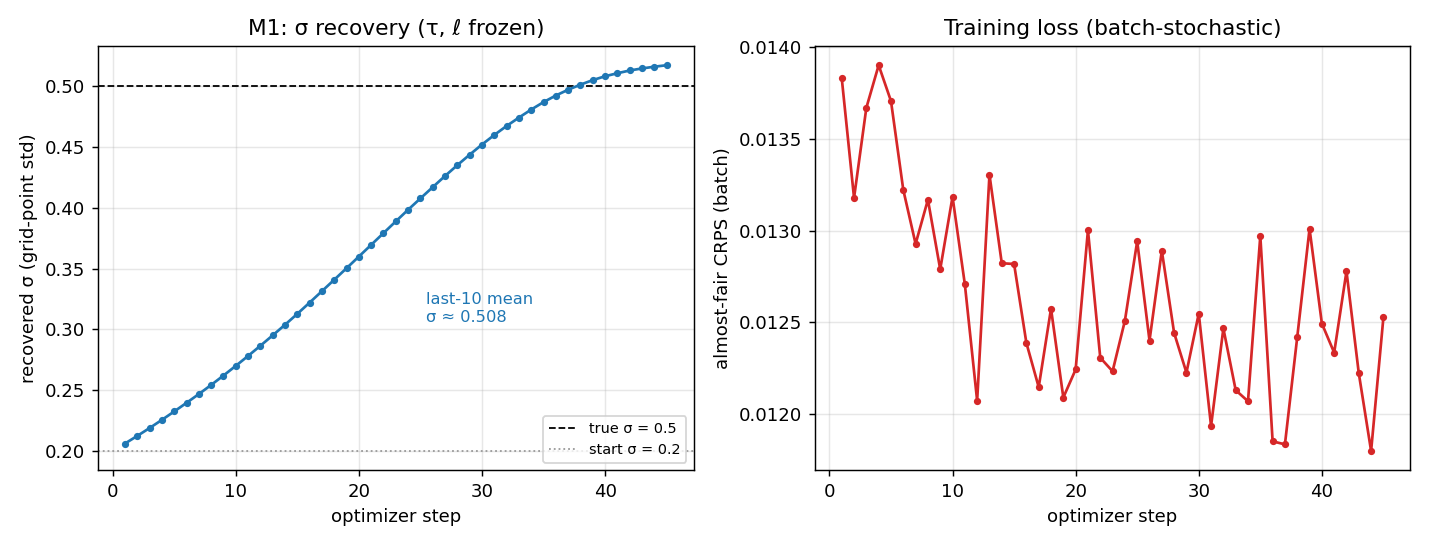
\includegraphics[width=\textwidth]{figures/fig_convergence.png}
\caption{\textbf{Left:} the recovered $\sigma$ versus optimiser step. Starting
from the wrong value 0.2 (dotted), $\sigma$ rises along a smooth, decelerating,
monotone curve, crosses the true 0.5 (dashed) near step~38, and plateaus at
$\approx 0.51$ (mean of the last ten steps $=0.508$; final value $0.517$) with no
overshoot. \textbf{Right:} the training loss. It is \emph{batch-stochastic} ---
each step scores a different random 3-case batch with its own common-random-number
draw --- so it wobbles and must \emph{not} be read as a smooth descent. The
parameter trajectory, not the raw loss, is the convergence signal.}
\label{fig:conv}
\end{figure}

Figure~\ref{fig:conv} is the headline evidence that the learning machinery works:
the gradient of an ensemble score, taken through a multi-day stochastic
integration by reverse-mode autodiff, points in the right direction and Adam
walks $\sigma$ from 0.2 to the neighbourhood of the truth. The $\approx 2\%$
residual is the finite-sample bias of \S\ref{sec:whybias}, not an error.

\subsection{The recovered $\sigma$ gives a calibrated ensemble}

\begin{figure}[h]
\centering
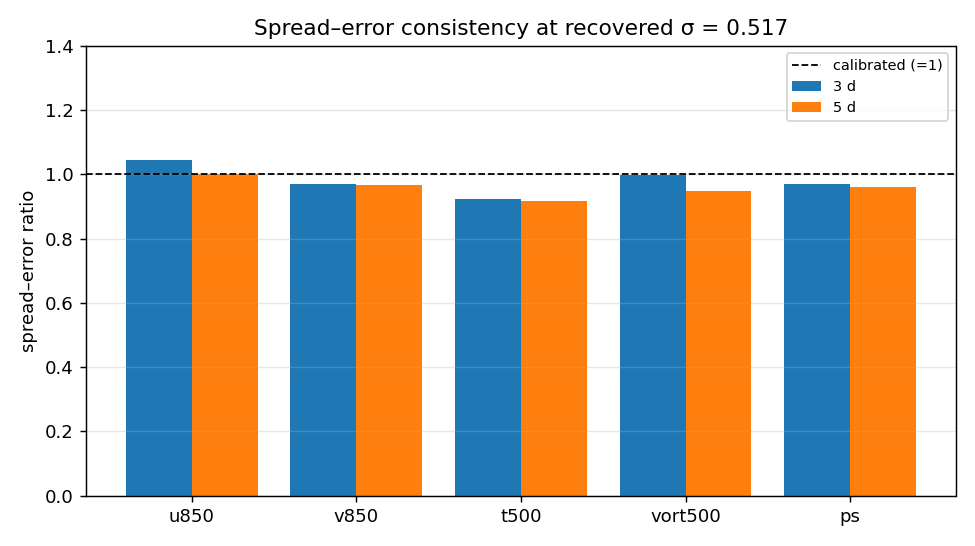
\includegraphics[width=0.85\textwidth]{figures/fig_spread_error.png}
\caption{Spread--error ratio \eqref{eq:sprerr} at the recovered $\sigma=0.517$,
for the five verification fields at 3- and 5-day leads, on the independent seed-1
dataset. All values lie in $[0.92, 1.05]$; the dashed line is the calibrated
target 1. The ensemble is very slightly \emph{under}-dispersed for \code{t500}
($\approx 0.92$) --- consistent with $\sigma$ tuned at a 1-day lead being a hair
low for the mid-tropospheric temperature spread at 3--5 days --- but is within the
calibrated band for every field.}
\label{fig:spr}
\end{figure}

\begin{table}[h]
\centering
\caption{Spread--error ratios behind Figure~\ref{fig:spr} (target $=1$).}
\label{tab:spr}
\begin{tabular}{lccccc}
\toprule
lead & u850 & v850 & t500 & vort500 & ps \\
\midrule
3 d & 1.045 & 0.971 & 0.924 & 0.998 & 0.971 \\
5 d & 1.001 & 0.966 & 0.917 & 0.947 & 0.960 \\
\bottomrule
\end{tabular}
\end{table}

\begin{figure}[h]
\centering
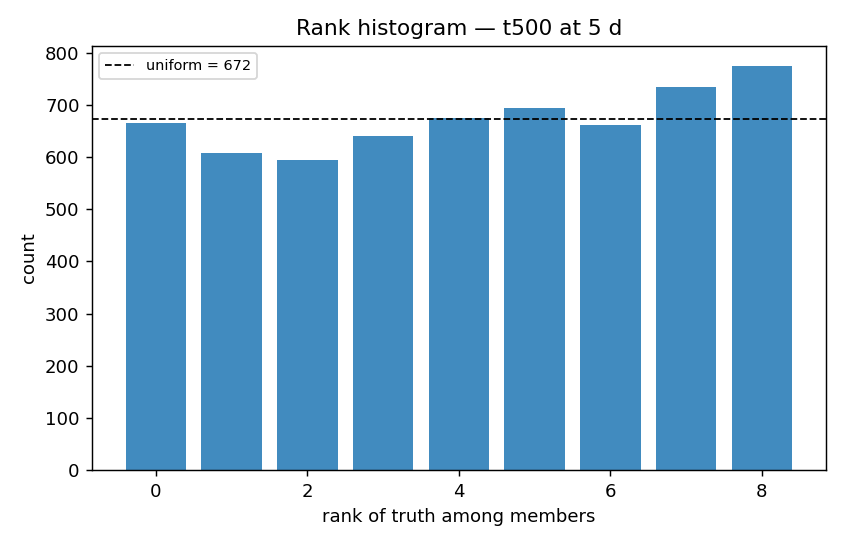
\includegraphics[width=0.49\textwidth]{figures/fig_rank_hist.png}
\hfill
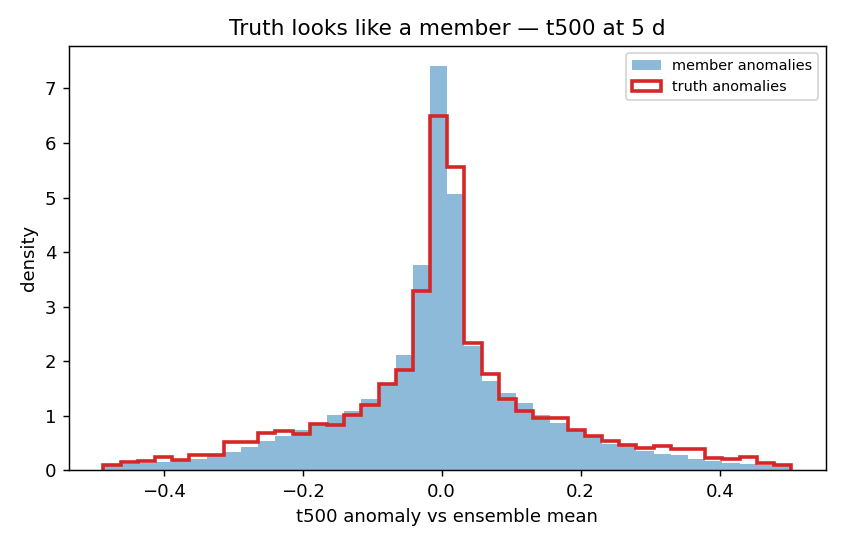
\includegraphics[width=0.49\textwidth]{figures/fig_anomaly_overlay.png}
\caption{\textbf{Left:} rank histogram of \code{t500} at 5 days (uniform level
$\approx 672$ per bin). It is approximately flat with a mild upward tilt towards
the higher ranks --- the same slight under-dispersion (and a hint of asymmetry)
seen in Table~\ref{tab:spr} --- but far from the deep $\cup$ shape of a badly
under-dispersed ensemble. \textbf{Right:} the distribution of the members'
\code{t500} anomalies (filled) with the truth's anomalies overlaid (outline). The
truth is a touch more peaked but tracks the member distribution closely: the truth
looks like another draw from the ensemble.}
\label{fig:rank}
\end{figure}

\begin{figure}[h]
\centering
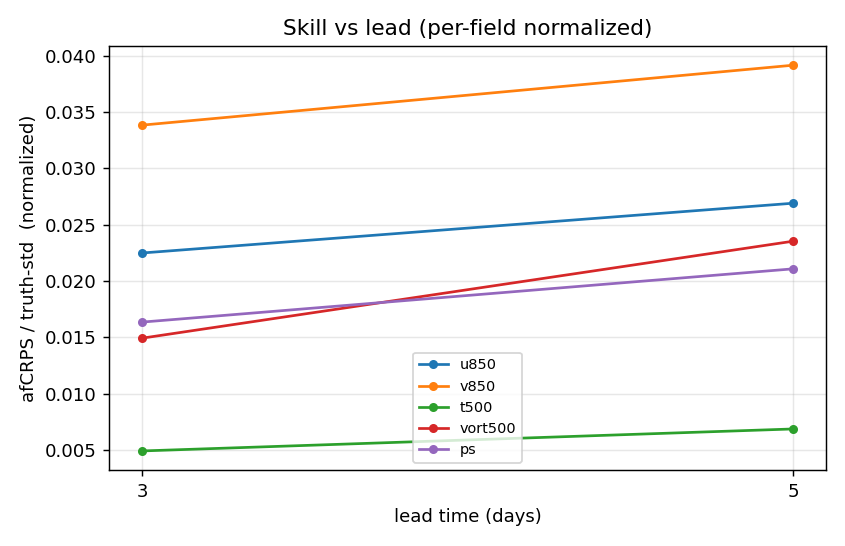
\includegraphics[width=0.62\textwidth]{figures/fig_afcrps_vs_lead.png}
\caption{afCRPS versus lead time, \emph{normalised per field by the truth
standard deviation} (the scaling used in the training loss, and the fix to an
earlier panel that plotted the score unnormalised and was visually dominated by
surface pressure in Pa). Skill degrades gracefully from 3 to 5 days, as expected.}
\label{fig:afcrps}
\end{figure}

Taken together, Figures~\ref{fig:conv}--\ref{fig:afcrps} confirm milestone~M1 on
two fronts: the optimiser \emph{recovers} the parameter, and the recovered
parameter \emph{produces a calibrated ensemble} on independent data.

%==============================================================================
\section{How the figures were made}\label{sec:repro}
%==============================================================================

Every figure is reproduced by three small scripts in
\code{examples/stochastic\_sppt/figures/} (all forcing float64+CPU at import):

\begin{description}
\item[\code{run\_sweep.py}] builds the T21 identical-twin training dataset
  (cached to \code{\_artifacts/}), then runs the $\sigma$-only recovery sweep. It
  freezes $\tau,\ell$ by \emph{masking} their gradients, checkpoints
  \code{\{step, params, opt\_state, history\}} every step, and honours a wall-clock
  budget so it is resumable:
  \begin{lstlisting}
def _sigma_only(grads):                 # keep only the log_sigma gradient
    return grads.replace(log_tau=jnp.zeros_like(grads.log_tau),
                         log_len=jnp.zeros_like(grads.log_len))
# ... each step: loss, grads = grad_fn(...); grads = _sigma_only(grads); adam.update(...)
# ... pickle {step, params, opt_state, history} to _artifacts/sweep_ckpt.pkl
  \end{lstlisting}
\item[\code{run\_calibration.py}] generates a fresh seed-1 dataset and runs
  forward-only ensembles at the recovered $\sigma$ (read from the sweep
  checkpoint), computing the spread--error ratios, rank histogram, and anomaly
  distributions, saved to \code{calib\_results.pkl}.
\item[\code{plot.py}] is pure \code{numpy}/\code{matplotlib} --- no \code{JAX} ---
  and renders all five PNGs from the two saved artifacts. Separating slow compute
  from fast plotting means a figure can be re-styled in a second.
\end{description}

To reproduce from scratch (from the repository root):
\begin{lstlisting}[language=bash]
python -m examples.stochastic_sppt.figures.run_sweep       --data-only
python -m examples.stochastic_sppt.figures.run_calibration --data-only
# run the sweep; re-invoke until it prints DONE (resumes from its checkpoint):
python -m examples.stochastic_sppt.figures.run_sweep --target-steps 45 --budget-seconds 520
python -m examples.stochastic_sppt.figures.run_calibration
python -m examples.stochastic_sppt.figures.plot
\end{lstlisting}

%==============================================================================
\section{Limitations and open questions}
%==============================================================================
\begin{itemize}
\item \textbf{Only $\sigma$ was recovered.} Recovering $\tau$ and $\ell$ jointly
  is harder: $\tau$ and $\ell$ are more weakly identified by a short-lead score
  than $\sigma$ is, and the three interact through $F_0$ \eqref{eq:F0}. This is
  the obvious next experiment.
\item \textbf{Mode~B (real model error)} --- training SPPT so a coarse ensemble
  covers the error against a higher-resolution truth --- is the milestone that
  matters for applications, and needs a GPU/cluster.
\item \textbf{Resolution dependence of $\sigma$} (\S\ref{sec:pattern}) should be
  removed if a learned $\sigma$ is to be read as a physical grid-point standard
  deviation across resolutions.
\item \textbf{The finite-sample bias} in $\sigma$ is understood
  (\S\ref{sec:whybias}) but not eliminated; multi-draw truth is the remedy.
\end{itemize}

%==============================================================================
\section{Exercises}
%==============================================================================
\begin{enumerate}
\item\label{ex:multidraw} \textbf{Multi-draw truth.} Modify \code{generate\_data.py}
  to store $K$ independent truth draws per case, and average the afCRPS over them
  in the loss. Measure the recovered $\sigma$ and its scatter as a function of
  $K\in\{1,2,4,8\}$. Confirm the plateau moves towards 0.5 and quantify the extra
  data-generation and per-step training cost --- verifying the claim in
  \S\ref{sec:data} that truth draws are cheap at training time.
\item\label{ex:cv} \textbf{A proper split.} Hold out a third dataset (seed 2) as a
  true test set; use seed 1 only to choose the learning rate and $\alpha$; report
  the final calibration on seed 2. Does the conclusion change?
\item \textbf{Joint recovery.} Unfreeze $\tau$ and $\ell$. Start from wrong values
  for all three and see which are recovered and which are not. Relate identifiability
  to lead time (try a longer lead if you have a GPU).
\item \textbf{Overshoot vs.\ bias.} Reproduce the lr $=0.1$ overshoot and confirm
  it is momentum, not sampling, by turning momentum off (plain SGD).
\item \textbf{Break the fairness correction.} Replace \eqref{eq:faircrps} with the
  naive $1/M^2$ estimator and watch the ensemble collapse (recovered $\sigma$ far
  too small) --- a hands-on demonstration of why fair CRPS matters.
\end{enumerate}

%==============================================================================
\section*{Further reading}
\addcontentsline{toc}{section}{Further reading}
%==============================================================================
\begin{itemize}
\item \textbf{SPPT and the pattern generator:} \citet{palmer2009} (the scheme is
  reproduced from its Appendix~8.1); \citet{leutbecher2017} for the modern
  SPPT/SKEB state of the art.
\item \textbf{Scoring rules:} \citet{gneiting2007} (proper scoring rules, the
  definitive reference); \citet{hersbach2000} (CRPS for ensemble systems);
  \citet{leutbecher2018} and \citet{lang2024} (fair / almost-fair CRPS).
\item \textbf{Calibration diagnostics:} \citet{hamill2001} (rank histograms and
  their pitfalls); \citet{fortin2014} (the spread--error relation done correctly).
\item \textbf{Stochastic gradients:} \citet{mohamed2020} (a superb survey of
  Monte-Carlo gradient estimation, including the reparameterization vs.\
  score-function distinction); \citet{kingma2014} (reparameterization in context);
  \citet{kingma2015adam} (Adam).
\item \textbf{The idealised model:} \citet{heldsuarez1994}.
\end{itemize}

%==============================================================================
\begin{thebibliography}{99}
\bibitem[Fortin et al.(2014)]{fortin2014} Fortin, V., Abaza, M., Anctil, F., \&
  Turcotte, R. (2014). Why should ensemble spread match the RMSE of the ensemble
  mean? \emph{Journal of Hydrometeorology}, 15(4), 1708--1713.
\bibitem[Gneiting \& Raftery(2007)]{gneiting2007} Gneiting, T., \& Raftery, A. E.
  (2007). Strictly proper scoring rules, prediction, and estimation.
  \emph{Journal of the American Statistical Association}, 102(477), 359--378.
\bibitem[Hamill(2001)]{hamill2001} Hamill, T. M. (2001). Interpretation of rank
  histograms for verifying ensemble forecasts. \emph{Monthly Weather Review},
  129(3), 550--560.
\bibitem[Held \& Suarez(1994)]{heldsuarez1994} Held, I. M., \& Suarez, M. J.
  (1994). A proposal for the intercomparison of the dynamical cores of atmospheric
  general circulation models. \emph{Bulletin of the AMS}, 75(10), 1825--1830.
\bibitem[Hersbach(2000)]{hersbach2000} Hersbach, H. (2000). Decomposition of the
  continuous ranked probability score for ensemble prediction systems.
  \emph{Weather and Forecasting}, 15(5), 559--570.
\bibitem[Kingma \& Welling(2014)]{kingma2014} Kingma, D. P., \& Welling, M.
  (2014). Auto-encoding variational Bayes. \emph{ICLR}. (The reparameterization
  trick.)
\bibitem[Kingma \& Ba(2015)]{kingma2015adam} Kingma, D. P., \& Ba, J. (2015).
  Adam: A method for stochastic optimization. \emph{ICLR}.
\bibitem[Lang et al.(2024)]{lang2024} Lang, S., et al. (2024). AIFS-CRPS:
  ensemble forecasting using a model trained with an almost-fair CRPS.
  \emph{npj Climate and Atmospheric Science / arXiv:2412.15832}.
\bibitem[Leutbecher et al.(2017)]{leutbecher2017} Leutbecher, M., et al. (2017).
  Stochastic representations of model uncertainties at ECMWF: state of the art and
  future vision. \emph{Quarterly Journal of the RMS}, 143(707), 2315--2339.
\bibitem[Leutbecher(2018)]{leutbecher2018} Leutbecher, M. (2019). Ensemble size:
  How suboptimal is less than infinity? \emph{Quarterly Journal of the RMS}, 145,
  107--128. (Fair scores for finite ensembles.)
\bibitem[Mohamed et al.(2020)]{mohamed2020} Mohamed, S., Rosca, M., Figurnov, M.,
  \& Mnih, A. (2020). Monte Carlo gradient estimation in machine learning.
  \emph{Journal of Machine Learning Research}, 21(132), 1--62.
\bibitem[Palmer et al.(2009)]{palmer2009} Palmer, T. N., Buizza, R., Doblas-Reyes,
  F., Jung, T., Leutbecher, M., Shutts, G. J., Steinheimer, M., \& Weisheimer, A.
  (2009). Stochastic parametrization and model uncertainty. \emph{ECMWF Technical
  Memorandum} 598.
\end{thebibliography}

\end{document}
